\section{Analog Filters}

\paragraph{a)}
The matlab function \textit{ellipord} was used to find the minimum order of a filter that meets
the specification. The minimum order of the filter is 7. A plot of the magnitude, phase, group delay and
the s-plane can be found in Figures \ref{fig:2_a_bode} - \ref{fig:2_a_pzmap}.

\paragraph{b)}

The filter was designed to have a minimum stop-band attenuation of 60dB and the stop band starts
at 24kHz. Therefore, we can be sure that all frequencies above 24kHz will be attenuated by at least 60dB.
To make sure that all aliasing-components are below 60dB, we have to use a sampling frequency of at least
$2*24kHz = 48kHz$.

\textbf{NOTE:} From the bode diagram, you can see that the actual frequency response, is ``better'' than
the specification. The 60dB stop-band attenuation is already reached at a frequency below 24 kHz.
In the calculation above, we assumed that the stop-band ``starts'' at 24 kHz. For this reason we have
some kind of reserve. For instance the frequency response may change a little bit due to quantization of the coefficients.

\paragraph{c)}

Like in task \textbf{a}, matlab was used to find the filter coefficients for the same specification,
but with a filter order fixed to 4. From the bode diagram in Figure \ref{fig:2_c_bode}, you
can see that all frequencies above approximately $51.5 kHz$ have an attenuation of more the 60dB.
So, for this filter, we have to use a sampling frequency of $2 \* 51.5 kHz = 103 kHz$ to 
achieve an attenuation of 60 dB for out-of-band distortion.

\begin{figure}[h!]
 \centering
 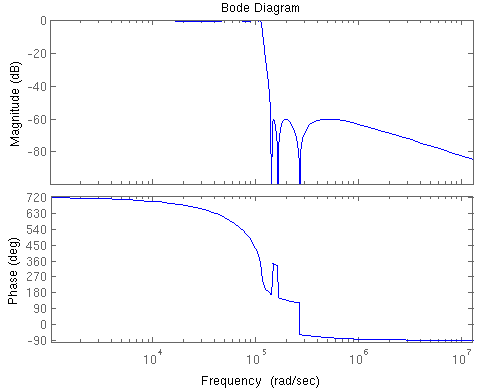
\includegraphics[width=0.8\textwidth]{./pics/2_a_bode.png}
 % 2_a_bode.png: 560x420 pixel, 90dpi, 15.81x11.85 cm, bb=0 0 448 336
 \label{fig:2_a_bode}
 \caption{Bode Diagram for task \textbf{a}: You can see in the bode diagram, that the designed filter, meets the specification.
 The filter has a ripple in the stop-band and the pass-band. The ripple in the stop-band comes from
 the zero points of the filter. The drawback of this fast stop-passband transition is the ripple
 and a very bad group delay (non linear phase).}
\end{figure}

\begin{figure}[h!]
 \centering
 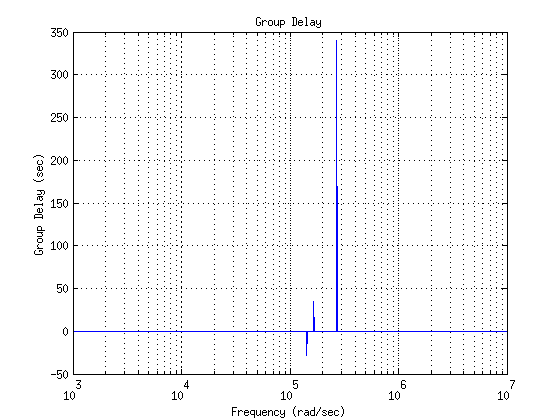
\includegraphics[width=0.8\textwidth]{./pics/2_a_grpdelay_2.png}
 % 2_a_bode.png: 560x420 pixel, 90dpi, 15.81x11.85 cm, bb=0 0 448 336
 \label{fig:2_a_grpdelay}
\end{figure}

\begin{figure}[h!]
 \centering
 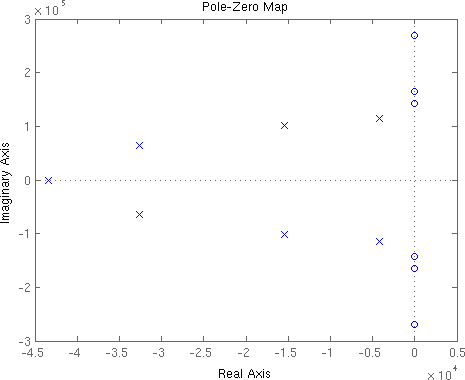
\includegraphics[width=0.8\textwidth]{./pics/2_a_pzmap.png}
 % 2_a_bode.png: 560x420 pixel, 90dpi, 15.81x11.85 cm, bb=0 0 448 336
 \caption{You can see that the filter consists of poles and zeros. All poles are on the left plane, which
 means the filter is stable.}
 \label{fig:2_a_pzmap}
\end{figure}

\begin{figure}[h!]
 \centering
 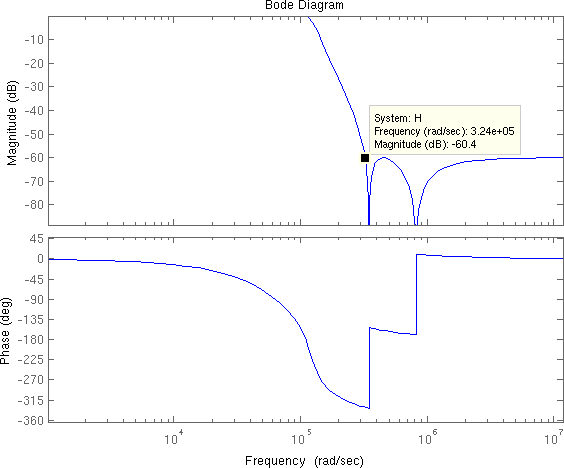
\includegraphics[width=\textwidth]{./pics/2_c_bode.png}
 % 2_a_bode.png: 560x420 pixel, 90dpi, 15.81x11.85 cm, bb=0 0 448 336
 \label{fig:2_c_bode}
 \caption{Bode Diagram for task \textbf{c}: You can see in the bode diagram, that the stop-band of the filter (60dB attenuation)
 starts at approximately $51.5 kHz$.}
\end{figure}



